\subsection{Helium and Beryllium}
The closed shell Helium and Beryllium calculations are presented in \cref{tab:res:helium_and_beryllium}, with relative errors compared to FCI in \cref{tab:res:helium_and_beryllium_percent_error}. For both HF add CCD in both restricted and unrestricted schemes, no problems of convergence was encountered. Adding a mixing parameter $p > 0$ for CCD only resulted in slower convergence.

\begin{table}[H]
    \centering
    \begin{tabular}{cccccc}
    \toprule
        Atom      &  $\Eref$ & CI & FCI & HF & RHF\\
    \midrule
    He & -2.7500 & -2.8385 & -2.9037 & -2.8311 & -2.8311 \\
    Be & -13.7160 & -14.3621 & -14.6674 & -14.5083 & -14.5083 \\
    \bottomrule
    \end{tabular}
    \newline
    \vspace*{10px}
    \newline
    \begin{tabular}{ccccc}
        \toprule
        Atom & CCD & RCCD & CCD(HF) & RCCD(HF) \\
        \midrule
        He & -2.7516 & -2.7516 & -2.8391 & -2.8391 \\
        Be & -13.7195 & -13.7195 & -14.5129 & -14.5129 \\
        \bottomrule
    \end{tabular}
    \caption{Ground state energies for Helium and Beryllium in \au\hspace{2px}Calculations done with configuration interaction with both singles and no constraints (full), in addition to HF and CCD in both restricted and unrestricted schemes. }\label[tab]{tab:res:helium_and_beryllium}
\end{table}

\begin{table}[H]
    \centering
    \begin{tabular}{ccccc}
    \toprule
    Atom      &  $\Eref$ & CI  & HF & RHF\\
    \midrule
    He & 5.29 & 2.25  & 2.50 & 2.50 \\
    Be & 6.49 & 2.08  & 1.09 & 1.09 \\
    \bottomrule
    \end{tabular}
    \newline
    \vspace*{10px}
    \newline
    \begin{tabular}{ccccc}
        \toprule
        Atom & CCD & RCCD & CCD(HF) & RCCD(HF) \\
        \midrule
        He & 5.24 & 5.24 & 2.22 & 2.22 \\
        Be & 6.46 & 6.46 & 1.05 & 1.05 \\
        \bottomrule
    \end{tabular}
    \caption{ Relative error in \% for Helium and Beryllium from \cref{tab:res:helium_and_beryllium}, using the FCI results as the exact energies. }\label[tab]{tab:res:helium_and_beryllium_percent_error}
\end{table}

\subsection{Harmonic Oscillator}
Comparing with the analytical case of two interacting particles at $\omega = 1.0$ having an energy of $3.00$, the best results was achieved when using the 12 first shells as basis states. Here HF, CCD with HO basis and CCD with HF basis produced energies off (relative error) 3.161909 (5.397\%), 3.089302 (2.977\%) and 3.005879 (0.196\%) respectively. This gave a clear sign that the basis and algorithm implementations were set up correctly. The results from the restricted and unrestricted schemes were again identical.

A comparison of the elapsed time for each algorithm to converge is presented in \cref{fig:res:timing}. All runs were made using $N=2$. For $R > 9$, the unrestricted implementation begun slowing down substantially.  

\begin{figure}[H]
    \centering
    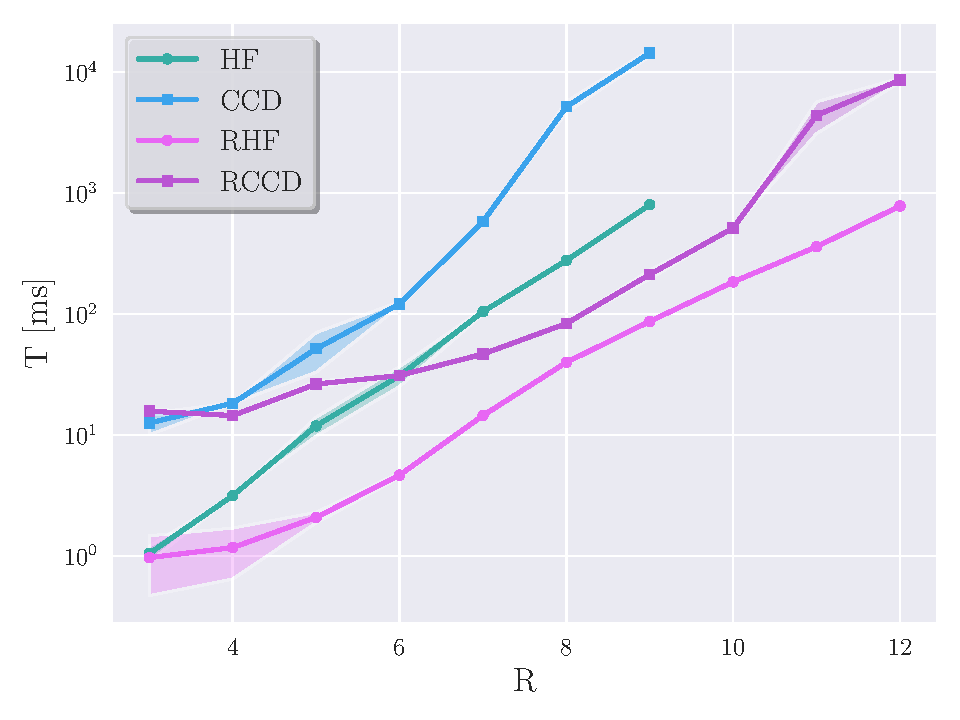
\includegraphics[width=\linewidth]{figs/timing.pdf}
    \caption{Showing elapsed time in milliseconds, comparing HF and CCD between the unrestricted and restricted schemes. $N=2$ particles were used, with time being averaged over ten runs. The shaded regions display the standard deviation over the ten runs.}\label[fig]{fig:res:timing}
\end{figure}
 Due to the computational expense when using a large amount of virtual states, all other energy calculations were done in the restricted scheme.  


Increasing the number of particles in the $\omega = 1.0$ system is presented in \cref{tab:res:ho_omega1}. For 12 and 20 particles, convergence for CCD using the HO basis was troublesome. This was in contrast to the HF basis, where no tuning of the mixing parameter was required. 

Lowering the frequency to $\omega = 0.5$, we show the same particle systems in \cref{tab:res:ho_omega0.5}. The convergence troubles still stood for the HO basis, but begun for smaller systems with a smaller number of virtual basis states. Here the 20 particle case also required tuning the mixing parameter for the HF basis, with $R > 7$ not achieving convergence with the parameters tested.
Lastly lowering the frequency all the way down to $\omega = 0.1$, the 2 and 6 particle systems are presented in \cref{tab:res:ho_omega0.1}. Using 12 and 20 particles did not result in any convergence and are therefor not shown.
\clearpage
% omega = 1.0 tables
\begin{table*}
    \begin{subtable}[h]{0.45\textwidth}
        \centering
        \begin{tabular}{cccc}
            \toprule
            $R$ & HF & CCD & CCD(HF) \\
            \midrule
            1 & 3.253314 & 3.253314 & 3.253314 \\
            2 & 3.253314 & 3.152329 & 3.152329 \\
            3 & 3.162691 & 3.141828 & 3.039049 \\
            4 & 3.162691 & 3.118684 & 3.025277 \\
            5 & 3.161921 & 3.110972 & 3.017946 \\
            6 & 3.161921 & 3.103343 & 3.013924 \\
            7 & 3.161909 & 3.099330 & 3.011408 \\
            8 & 3.161909 & 3.095925 & 3.009624 \\
            9 & 3.161909 & 3.093663 & 3.008351 \\
            10 & 3.161909 & 3.091818 & 3.007366 \\
            11 & 3.161909 & 3.090438 & 3.006599 \\
            12 & 3.161909 & 3.089302 & 3.005979 \\
            \bottomrule
        \end{tabular}
        \caption{$N = 2$}\label[tab]{tab:res:ho_omega1_N2}
    \end{subtable}
    \hfill
    \begin{subtable}[h]{0.45\textwidth}
        \centering
        \begin{tabular}{ccccc}
            \toprule
            $R$ & $p$ & HF & CCD & CCD(HF) \\
            \midrule
            2 & N & 22.219813 & 22.219813 & 22.219813 \\
            3 & N & 21.593198 & 21.974680 & 21.423816 \\
            4 & N & 20.766919 & 21.854198 & 20.429269 \\
            5 & N & 20.748402 & 21.793640 & 20.332466 \\
            6 & N & 20.720257 & 21.750086 & 20.274029 \\
            7 & N & 20.720132 & 21.718843 & 20.249851 \\
            8 & N & 20.719248 & 21.695225 & 20.234708 \\
            9 & 0.30 & 20.719248 & 21.675965 & 20.224387 \\
            10 & 0.30 & 20.719217 & 21.661863 & 20.217073 \\
            11 & 0.30 & 20.719215 & 21.649847 & 20.211538 \\
            12 & 0.30 & 20.719215 & 21.640798 & 20.207259 \\
            \bottomrule
        \end{tabular}
        \caption{$N = 6$}\label[tab]{tab:res:ho_omega1_N6}
    \end{subtable}
    \hfill
    \begin{subtable}[h]{0.45\textwidth}
        \centering
        \begin{tabular}{ccccc}
            \toprule
            $R$ & $p$ & HF & CCD & CCD(HF) \\
            \midrule
            3 & $>$0.99 & 73.765549 & 73.765549 & 73.765549 \\
            4 & $>$0.99 & 70.673849 & - & 70.324257 \\
            5 & $>$0.99 & 67.569930 & - & 67.031101 \\
            6 & $>$0.99 & 67.296869 & - & 66.526674 \\
            7 & $>$0.99 & 66.934745 & - & 66.049566 \\
            8 & $>$0.99 & 66.923094 & - & 65.972154 \\
            9 & $>$0.99 & 66.912244 & - & 65.921206 \\
            10 & $>$0.99 & 66.912035 & - & 65.889282 \\
            11 & $>$0.99 & 66.911365 & - & 65.866717 \\
            12 & $>$0.99 & 66.911364 & - & 65.849773 \\
        \bottomrule
    \end{tabular}
    \caption{$N = 12$}\label[tab]{tab:res:ho_omega1_N12}
\end{subtable}
    \hfill
    \begin{subtable}[h]{0.45\textwidth}
        \centering
        \begin{tabular}{ccccc}
            \toprule
            $R$ & $p$ & HF & CCD & CCD(HF) \\
            \midrule
            4 & $>$0.99 & 177.963297 & 177.963297 & 177.963297 \\
            5 & $>$0.99 & 168.808284 & - & 168.459454 \\
            6 & $>$0.99 & 161.339721 & - & 160.594508 \\
            7 & $>$0.99 & 159.958722 & - & 158.841116 \\
            8 & $>$0.99 & 158.400172 & - & 157.038328 \\
            9 & $>$0.99 & 208.177129 & - & 156.676039 \\
            10 & $>$0.99 & 158.017667 & - & 156.367932 \\
            11 & $>$0.99 & 158.010276 & - & 156.292420 \\
            12 & $>$0.99 & 158.004951 & - & 156.238255 \\
            \bottomrule
        \end{tabular}
        \caption{$N = 20$}\label[tab]{tab:res:ho_omega1_N20}
    \end{subtable}
    \caption{Showing ground state energies for $\omega = 1.0$, when increasing the number of shells $R$ used for the calculation up to and including $R=12$. The four entries \cref{tab:res:ho_omega1_N2},\cref{tab:res:ho_omega1_N6},\cref{tab:res:ho_omega1_N12} and \cref{tab:res:ho_omega1_N20} shows 2, 6, 12 and 20 particles respectively. Restricted schemes have been used for all calculations, with CCD and CCD(HF) using the HO and HF basis respectively. The column $p$ displays the mixing parameter for the HO basis used when convergence without it was not achieved, with `N` marking no mixing required. A dashed line `-` for the energy marks no convergence across different mixing parameters.}\label[tab]{tab:res:ho_omega1}
\end{table*}

% omega = 0.5 tables
\begin{table*}
    \begin{subtable}[h]{0.45\textwidth}
        \centering
        \begin{tabular}{cccc}
            \toprule
            $R$ & HF & CCD & CCD(HF) \\
            \midrule
            1 & 1.886227 & 1.886227 & 1.886227 \\
            2 & 1.886227 & 1.786915 & 1.786915 \\
            3 & 1.799856 & 1.778907 & 1.681981 \\
            4 & 1.799856 & 1.760121 & 1.673883 \\
            5 & 1.799748 & 1.754389 & 1.670056 \\
            6 & 1.799748 & 1.748238 & 1.667808 \\
            7 & 1.799745 & 1.745232 & 1.666479 \\
            8 & 1.799745 & 1.742551 & 1.665532 \\
            9 & 1.799743 & 1.740856 & 1.664848 \\
            10 & 1.799743 & 1.739446 & 1.664278 \\
            11 & 1.799742 & 1.738412 & 1.663866 \\
            12 & 1.799742 & 1.737563 & 1.663523 \\
            \bottomrule
        \end{tabular}
        \caption{$N = 2$}\label[tab]{tab:res:ho_omega0.5_N2}
    \end{subtable}
    \hfill
    \begin{subtable}[h]{0.45\textwidth}
        \centering
        \begin{tabular}{ccccc}
            \toprule
            $R$ & $p$ & HF & CCD & CCD(HF) \\
            \midrule
            2 & N & 13.640713 & 13.640713 & 13.640713 \\
            3 & N & 13.051620 & 13.385995 & 12.901525 \\
            4 & N & 12.357471 & 13.261110 & 12.057347 \\
            5 & $>$0.99 & 12.325128 & - & 11.935004 \\
            6 & $>$0.99 & 12.271499 & - & 11.864102 \\
            7 & $>$0.99 & 12.271375 & - & 11.849764 \\
            8 & $>$0.99 & 12.271361 & - & 11.841326 \\
            9 & $>$0.99 & 12.271337 & - & 11.835472 \\
            10 & $>$0.99 & 12.271326 & - & 11.831348 \\
            11 & $>$0.99 & 12.271324 & - & 11.828237 \\
            12 & $>$0.99 & 12.271320 & - & 11.825837 \\
            \bottomrule
        \end{tabular}
        \caption{$N = 6$}\label[tab]{tab:res:ho_omega0.5_N6}
    \end{subtable}
    \hfill
    \begin{subtable}[h]{0.45\textwidth}
        \centering
        \begin{tabular}{ccccc}
            \toprule
            $R$ & $p$ & HF & CCD & CCD(HF) \\
            \midrule
            3 & $>$0.99 & 46.361130 & 46.361130 & 46.361130 \\
            4 & $>$0.99 & 43.663267 & - & 43.309862 \\
            5 & $>$0.99 & 41.108851 & - & 40.654710 \\
            6 & $>$0.99 & 40.750512 & - & 40.068342 \\
            7 & $>$0.99 & 40.302719 & - & 39.508497 \\
            8 & $>$0.99 & 40.263752 & - & 39.399125 \\
            9 & $>$0.99 & 40.216688 & - & 39.329313 \\
            10 & $>$0.99 & 40.216252 & - & 39.309411 \\
            11 & $>$0.99 & 40.216195 & - & 39.296003 \\
            12 & $>$0.99 & 40.216165 & - & 39.285970 \\
            \bottomrule
        \end{tabular}
        \caption{$N = 12$}\label[tab]{tab:res:ho_omega0.5_N12}
    \end{subtable}
    \hfill
    \begin{subtable}[h]{0.5\textwidth}
        \centering
        \begin{tabular}{cccccc}
            \toprule
            $R$ & $p$ & $p(HF)$ & HF & CCD & CCD(HF) \\
            \midrule
            4 & $>$0.99 & N & 113.412648 & 113.412648 & 113.412648 \\
            5 & $>$0.99 & 0.20 & 105.227282 & - & 104.896465 \\
            6 & $>$0.99 & 0.20 & 99.754600 & - & 99.119518 \\
            7 & $>$0.99 & $>$0.99 & 131.446882 & - & - \\
            8 & $>$0.99 & $>$0.99 & 133.900840 & - & - \\
            9 & $>$0.99 & $>$0.99 & 134.132319 & - & - \\
            10 & $>$0.99 & $>$0.99 & 133.574242 & - & - \\
            11 & $>$0.99 & $>$0.99 & 133.244135 & - & - \\
            12 & $>$0.99 & $>$0.99 & 133.178089 & - & - \\
            \bottomrule
        \end{tabular}
        \caption{$N = 20$}\label[tab]{tab:res:ho_omega0.5_N20}
    \end{subtable}
    \caption{Showing ground state energies for $\omega = 0.5$, when increasing the number of shells $R$ used for the calculation up to and including $R=12$. The four entries \cref{tab:res:ho_omega0.5_N2},\cref{tab:res:ho_omega0.5_N6},\cref{tab:res:ho_omega0.5_N12} and \cref{tab:res:ho_omega0.5_N20} shows 2, 6, 12 and 20 particles respectively. Restricted schemes have been used for all calculations, with CCD and CCD(HF) using the HO and HF basis respectively. The columns $p$ and $p(HO)$ displays the mixing parameter used for the HO and HF basis respectively when convergence without it was not achieved, with `N` marking no mixing required. A dashed line `-` for the energy marks no convergence across different mixing parameters.}\label[tab]{tab:res:ho_omega0.5}
\end{table*}

\begin{table*}    
    \begin{subtable}[h]{0.45\textwidth}
        \centering
        \begin{tabular}{cccccc}
            \toprule
            $R$ & $p$ & $p(HF)$ & HF & CCD & CCD(HF) \\
            \midrule
            1 & N & N & 0.596333 & 0.596333 & 0.596333 \\
            2 & N & N & 0.596333 & 0.512521 & 0.512521 \\
            3 & N & N & 0.526903 & 0.505981 & 0.442244 \\
            4 & N & N & 0.526903 & 0.499233 & 0.442018 \\
            5 & 0.30 & N & 0.525666 & 0.497206 & 0.443337 \\
            6 & 0.30 & N & 0.525666 & 0.494263 & 0.443147 \\
            7 & 0.30 & N & 0.525635 & 0.493172 & 0.443050 \\
            8 & 0.30 & N & 0.525635 & 0.498285 & 0.442974 \\
            9 & 0.30 & N & 0.525635 & 0.491290 & 0.442921 \\
            10 & 0.30 & N & 0.525635 & 0.490676 & 0.442887 \\
            11 & 0.50 & N & 0.525635 & 0.490305 & 0.442856 \\
            12 & 0.50 & 0.30 & 0.525635 & 0.489960 & 0.442849 \\
            \bottomrule
        \end{tabular}
        \caption{$N = 2$}\label[tab]{tab:res:ho_omega0.1_N2}
    \end{subtable}
    \hfill
    \begin{subtable}[h]{0.45\textwidth}
        \centering
        \begin{tabular}{cccccc}
            \toprule
            $R$ & $p$ & $p(HF)$ & HF & CCD & CCD(HF) \\
            \midrule
            2 & $>$0.99 & N & 4.864244 & 4.864244 & 4.864244 \\
            3 & $>$0.99 & N & 4.435740 & - & 4.319916 \\
            4 & $>$0.99 & N & 4.019787 & - & 3.829968 \\
            5 & $>$0.99 & N & 3.963148 & - & 3.666723 \\
            6 & $>$0.99 & N & 3.870617 & - & 3.597876 \\
            7 & $>$0.99 & 0.30 & 3.863135 & - & 3.590411 \\
            8 & $>$0.99 & 0.30 & 3.852880 & - & 3.587734 \\
            9 & $>$0.99 & 0.30 & 3.852591 & - & 3.587314 \\
            10 & $>$0.99 & 0.30 & 3.852393 & - & 3.587159 \\
            11 & $>$0.99 & 0.30 & 3.852391 & - & 3.586844 \\
            12 & $>$0.99 & 0.30 & 3.852382 & - & 3.586606 \\
            \bottomrule
        \end{tabular}
        \caption{$N = 6$}\label[tab]{tab:res:ho_omega0.1_N6}
    \end{subtable}
    \caption{Showing ground state energies for $\omega = 1.0$, when increasing the number of shells $R$ used for the calculation up to and including $R=12$. The four entries \cref{tab:res:ho_omega0.1_N2} and \cref{tab:res:ho_omega0.1_N6} shows 2 and 6 particles respectively. Restricted schemes have been used for all calculations, with CCD and CCD(HF) using the HO and HF basis respectively. The columns $p$ and $p(HO)$ displays the mixing parameter used for the HO and HF basis respectively when convergence without it was not achieved, with `N` marking no mixing required. A dashed line `-` for the energy marks no convergence across different mixing parameters.}\label[tab]{tab:res:ho_omega0.1}
\end{table*}
\clearpage